\documentclass[12pt, letterpaper]{article}

% ==========================================
%              DOCUMENT PACKAGES
% ==========================================

% --- Core Language & Encoding ---
\usepackage[english]{babel} % Sets the language and regional settings for English documents
\usepackage[utf8]{inputenc} % Allows the use of UTF-8 characters in the document
\usepackage[T1]{fontenc} % Specifies the font encoding
\usepackage[margin=2cm]{geometry} % Sets the page margins

% --- Colors & Graphics ---
\usepackage[table,dvipsnames]{xcolor} % Advanced color management
% \usepackage{color} % Basic package for text and background colors
\usepackage{graphicx} % Enhanced support for including external images and scaling them
\usepackage{adjustbox} % Adjusts the size, scaling, and alignment of boxes, images, and tables
% \usepackage{background} % Allows adding background images or watermarks to pages
\usepackage{float} % Improves the interface for floating objects and adds the [H] placement
\usepackage{pdflscape} % Makes landscape pages display correctly on screen in PDF viewers
\usepackage{pdfpages} % Allows the inclusion of external multi-page PDF documents

% --- Math, Science & Engineering ---
\usepackage{amsfonts} % Provides extended mathematical fonts
\usepackage{amsmath} % Provides advanced mathematical typesetting and environments
\usepackage{amssymb} % Provides extended mathematical symbols
% \usepackage{amsmath, amssymb} % (Redundant combination line omitted for stability)
\usepackage{amsthm} % Facilitates the creation of theorem-like environments
\usepackage{mathtools} % Enhances amsmath with additional math tools and bug fixes
\usepackage{thmtools} % Extensions and customization options for theorem environments
\usepackage{nicematrix} % Enhances matrices and tabulars using PGF/TikZ
\usepackage{xy} % Typesets complex graphs and diagrams
\usepackage{circuitikz} % Allows drawing of electrical networks and circuits

% --- Typography & Fonts ---
\usepackage{avant} % Sets the default sans-serif font to Avant Garde
\usepackage{cantarell} % Sets the default sans-serif font to Cantarell
\usepackage{charter} % Sets the default roman font to Charter
\usepackage{cmbright} % Sets the font family to Computer Modern Bright 
\usepackage{helvet} % Sets the default sans-serif font to Helvetica
\usepackage{inconsolata} % Sets the default typewriter (monospace) font to Inconsolata
\usepackage{iwona} % Sets the font family to Iwona 
\usepackage{kurier} % Sets the font family to Kurier 
\usepackage{lmodern} % Loads the Latin Modern fonts 
\usepackage{textcomp} % Provides additional text symbols
\usepackage{ulem} % Provides various types of text underlining and strikethroughs

% --- Tables & Lists ---
\usepackage{array} % Extends the array and tabular environments
% \usepackage{arydshln} % Conflicts with longtable
\usepackage{bigstrut} % Adds custom vertical space in table rows
\usepackage{booktabs} % Enhances the quality of tables with better horizontal rules
% \usepackage{colortbl} % Allows coloring of rows, columns, and individual cells in tables
\usepackage{diagbox} % Creates table cells with diagonal lines 
\usepackage{enumitem} % Provides advanced control over list environments
\usepackage{longtable} % Allows tables to break across multiple pages
\usepackage{multirow} % Allows individual table cells to span across multiple rows
\usepackage{tabularx} % Creates tables with dynamically adjustable-width columns
\usepackage{pgfplotstable} % Reads and cleanly formats numerical tables directly from CSV

% --- Formatting, Layout & UI ---
\usepackage{blindtext} % Generates dummy text for testing document layouts
\usepackage{caption} % Customizes captions in floating environments
\usepackage{comment} % Allows you to block out large sections of text
\usepackage{emptypage} % Automatically removes headers and footers on empty pages
\usepackage{fancyhdr} % Allows complete customization of headers and footers
\usepackage{fancyvrb} % Enhanced verbatim environments for writing raw code
\usepackage{framed} % Creates framed, shaded, or differently highlighted text regions
\usepackage{fullpage} % Quickly sets all page margins to 1 inch
\usepackage{lipsum} % Generates Lorem Ipsum dummy text
\usepackage{mdframed} % Creates highly customizable framed environments
\usepackage{multicol} % Allows intermixing single and multiple text columns
\usepackage{parskip} % Replaces standard paragraph indentation with vertical spacing
\usepackage{setspace} % Controls line spacing (single, one-and-a-half, double)
\usepackage{subcaption} % Supports sub-figures and sub-tables with independent captions
% \usepackage{subfig} % Older package for sub-figures (subcaption is generally preferred now)
\usepackage{tcolorbox} % Creates heavily customized colored and framed text boxes
\usepackage{titlesec} % Customizes the formatting of section, subsection, and chapter headings
\usepackage{titling} % Provides advanced control over the typesetting of the document title

% --- Bibliographies & References ---
\usepackage{biblatex} % Advanced, modern bibliographic processing and formatting
\usepackage{csquotes} % Context-sensitive quotation facilities
\usepackage{makeidx} % Supports the generation of a document index
% \usepackage{natbib} % Flexible bibliography support, particularly for author-year citation styles

% --- TikZ & Plotting ---
\usepackage{tikz} % Advanced package for creating vector graphics and diagrams programmatically
\usepackage{pgf-pie} % Draws pie charts programmatically using PGF/TikZ
\usepackage{pgfplots} % Creates high-quality mathematical plots, charts, and graphs
% \usepackage{fancytikzposter} % Used to create large format academic posters using TikZ

% --- URLs & Hyperlinks ---
\usepackage{url} % Formats and properly hyphenates long URLs
\usepackage{breakurl} % Allows line breaks in URLs, especially when compiled with latex -> dvips
\usepackage{hyperref} % Creates cross-referencing, clickable links, and PDF bookmarks

% --- Code Formatting ---
\usepackage{listings} % Typesets programming source code with formatting and syntax highlighting


% ==========================================
%           DOCUMENT CONFIGURATION
% ==========================================

% Custom color definitions
\definecolor{mygray}{gray}{0.9}

% Hyperlink configuration
\hypersetup{
    colorlinks=true,
    linkcolor=blue,
    urlcolor=blue
}

% Configuración adicional para breaks en URLs
\def\UrlBreaks{\do\/\do-\do_\do.\do=\do?\do\&}
\expandafter\def\expandafter\UrlBreaks\expandafter{\UrlBreaks\do\a\do\b\do\c\do\d\do\e\do\f\do\g\do\h\do\i\do\j\do\k\do\l\do\m\do\n\do\o\do\p\do\q\do\r\do\s\do\t\do\u\do\v\do\w\do\x\do\y\do\z}

%Uncomment the following lines to use a sans-serif font
%\usepackage{helvet}
%\renewcommand{\familydefault}{\sfdefault}

% TikZ libraries
\usetikzlibrary{shapes.geometric, positioning, decorations.pathreplacing}

\graphicspath{ {./img/} } % Sets the path for the graphics

\newlist{biblio}{enumerate}{1}
\setlist[biblio,1]{
    label=[\arabic*],
    leftmargin=2.2em,
    labelsep=0.5em,
    itemsep=0.35em,
    parsep=0pt,
    topsep=0.35em,
    align=left
}

\makeindex

% \tiny
% \scriptsize
% \footnotesize
% \small
% \normalsize (default size)
% \large
% \Large
% \LARGE
% \huge
% \Huge


% ==========================================
%         GLOBAL LISTINGS SETTINGS
% ==========================================
\lstset{
	basicstyle=\ttfamily\small,
	numbers=left,
	numberstyle=\tiny\color{gray},
	stepnumber=1,
	numbersep=10pt,
	backgroundcolor=\color{white},
	showspaces=false,
	showstringspaces=false,
	breaklines=true,
	frame=single,
	tabsize=2, 
    captionpos=b, 
    lineskip=-1pt,
	extendedchars=true,
	literate={á}{{\'a}}1 {é}{{\'e}}1 {í}{{\'i}}1 {ó}{{\'o}}1 {ú}{{\'u}}1 {Á}{{\'A}}1 {É}{{\'E}}1 {Í}{{\'I}}1 {Ó}{{\'O}}1 {Ú}{{\'U}}1 {ñ}{{\~n}}1 {Ñ}{{\~N}}1 {¿}{{\textquestiondown}}1 {¡}{{\textexclamdown}}1
}

% ==========================================
%            LANGUAGE: SQL
% ==========================================
\lstdefinestyle{sqlstyle}{
	language=SQL,
	keywordstyle=\color{blue}\bfseries,
	commentstyle=\color[rgb]{0,0.5,0}\itshape,
	stringstyle=\color{red}
}

% ==========================================
%            LANGUAGE: VHDL
% ==========================================
\lstdefinelanguage{VHDL}{
	morekeywords={entity, architecture, signal, port, in, out, inout, begin, end, process, if, then, else, elsif, case, when, others, for, while, loop, wait, library, use, std_logic, std_logic_vector, integer, boolean, rising_edge, falling_edge, component, generic, map, downto, to, and, or, not, xor, nand, nor, xnor},
	morecomment=[l]{--},
	morestring=[b]",
	sensitive=false,
	alsoletter={_}
}

\lstdefinestyle{vhdl}{
	language=VHDL,
	keywordstyle=\color{blue}\bfseries,
	commentstyle=\color[rgb]{0,0.6,0}\itshape,
	stringstyle=\color{red}
}

% ==========================================
%              LANGUAGE: C
% ==========================================
\lstdefinestyle{cstyle}{
	language=C,
	keywordstyle=\color{blue}\bfseries,
	commentstyle=\color[rgb]{0,0.5,0}\itshape,
	stringstyle=\color{red},
	directivestyle=\color{purple},
    tabsize=4 % Overrides the global tabsize of 2 for C code specifically
}

% ==========================================
%             LANGUAGE: C++
% ==========================================
\lstdefinestyle{cppstyle}{
	language=C++,
	keywordstyle=\color{blue}\bfseries,
	commentstyle=\color[rgb]{0,0.5,0}\itshape,
	stringstyle=\color{red},
	directivestyle=\color{purple},
    tabsize=4
}

% ==========================================
%           LANGUAGE: PYTHON
% ==========================================
\lstdefinestyle{pythonstyle}{
	language=Python,
	keywordstyle=\color{blue}\bfseries,
	commentstyle=\color[rgb]{0,0.5,0}\itshape,
	stringstyle=\color{red},
    % Python relies heavily on indentation, so keeping tabsize aligned is important
    tabsize=4
}

% ==========================================
%             LANGUAGE: BASH
% ==========================================
\lstdefinestyle{bashstyle}{
	language=bash,
	keywordstyle=\color{blue}\bfseries,
	commentstyle=\color[rgb]{0,0.5,0}\itshape,
	stringstyle=\color{red},
    % Bash variables often use $, so we can highlight them dynamically if needed
    moredelim=[s][\color{orange}]{\$\{}{\}}
}

% ==========================================
%           LANGUAGE: ASSEMBLY
% ==========================================
\lstdefinestyle{asmstyle}{
	language=[x86masm]Assembler,
	keywordstyle=\color{blue}\bfseries,
	commentstyle=\color[rgb]{0,0.5,0}\itshape,
	stringstyle=\color{red},
    % Adding common ARM/Microcontroller instructions for better highlighting
    morekeywords={ldr, str, mov, cmp, add, sub, b, bl, bx, push, pop, svc, eor, and, orr, lsl, lsr}
}

\usetikzlibrary{fit,tikzmark}

\begin{document}

\begin{titlepage}

	\begin{tikzpicture}[remember picture,overlay]
		\node[anchor=north west, inner sep=30] at (current page.north west) {
			
\includegraphics[width=3.5cm, height=4cm]{unam.png}
		};
		% \node[anchor=north west, inner sep=30] at (current page.north west) {
		% 	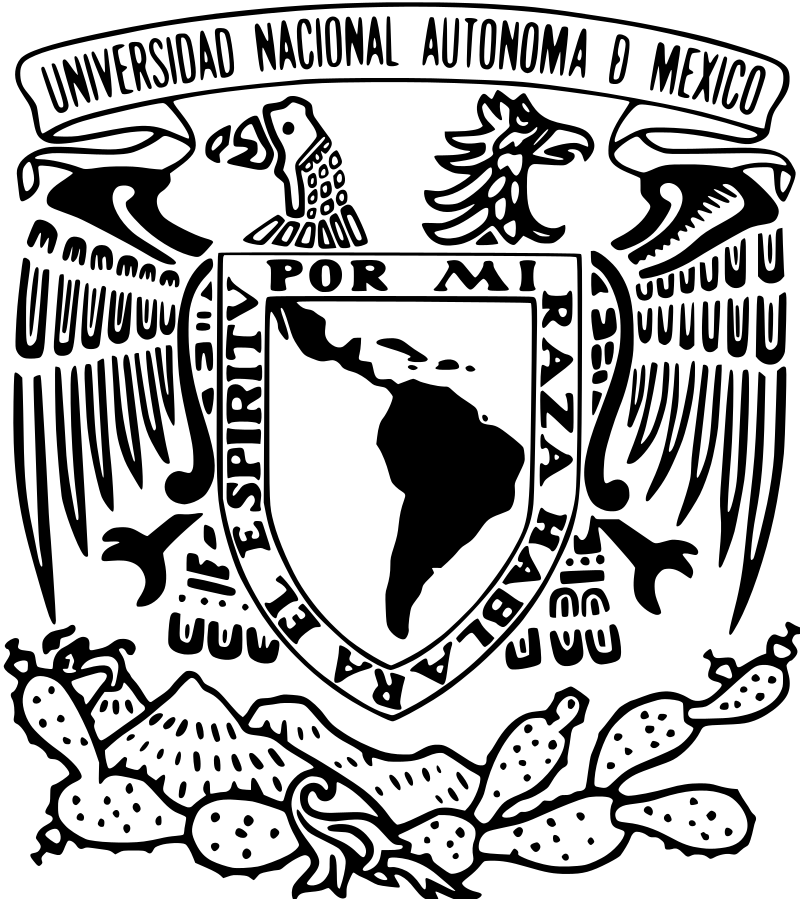
\includegraphics[width=4cm]{escudoUNAM_negro.png}
		% };

		\node[anchor=north east, inner sep=30] at (current page.north east) {
			
\includegraphics[width=3.5cm, height=4cm]{escudoFI_color.png}
		};
		% \node[anchor=north east, inner sep=30] at (current page.north east) {
		% 	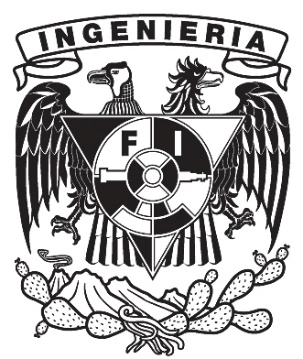
\includegraphics[width=4cm]{escudoFI_negro.png}
		% };
	\end{tikzpicture}

	\begin{center}
		\vspace*{2.5cm}

		\Large
		\textbf{UNIVERSIDAD NACIONAL AUTÓNOMA DE MÉXICO}\\
		\textbf{FACULTAD DE INGENIERÍA}\\
		\textbf{INGENIERÍA EN COMPUTACIÓN}\\

		\vspace*{1.5cm}
		\large
		\textbf{Laboratorio de Organización y Arquitectura de Computadoras}\\
		\large
		\vspace*{1cm}
		\textbf{Reporte - Secuenciador Básico}\\
		\vspace{1.5cm}
	\end{center}

	%grupo de la materia
	\large
	\textbf{INTEGRANTES EQUIPO 8:}
	\begin{itemize}
		\item Saldaña Navarrete Andrea - \textit{Grupo Teoria:} 2
		\item Tepal Briseño Hansel Yael - \textit{Grupo Teoria:} 1
		\item Ugartechea González Luis Antonio - \textit{Grupo Teoria:} 1
	\end{itemize}
	\vspace{2.5cm}

	\large
	%fecha de entrega
	\textbf{NOMBRE DELPROFESOR:} Ing. Diana Karen Pérez Pérez \\
	\textbf{GRUPO:} 06\\
	\textbf{SEMESTRE:} \underline{2027-1}\\
	\vspace{0.5cm}

	\begin{center}
		\textbf{FECHA DE ENTREGA:} 12 de noviembre del 2026\\
	\end{center}
\end{titlepage}


\section*{Objetivo}

Familiarizar al alumno en el conocimiento del secuenciador básico, el cual es una parte
fundamental del procesador.

\section*{Introducción}



\section*{Desarrollo}

\subsection*{1. Diseñe una carta ASM con las siguientes características:}

\begin{itemize}
    \item Estados: 14 a 16
    \item Entradas: 2: \texttt{INT} y \texttt{Qaux}
    \item Salidas: 4
    \begin{itemize}
        \item 2 con lógica estándar: $S_1$ y $S_0$
        \item 2 con lógica negada: $\overline{U_1}$ y $\overline{U_0}$
    \end{itemize}
\end{itemize}

\begin{figure}[H]
    \centering
    \begin{adjustbox}{width=\textwidth, height=\textheight, keepaspectratio}
    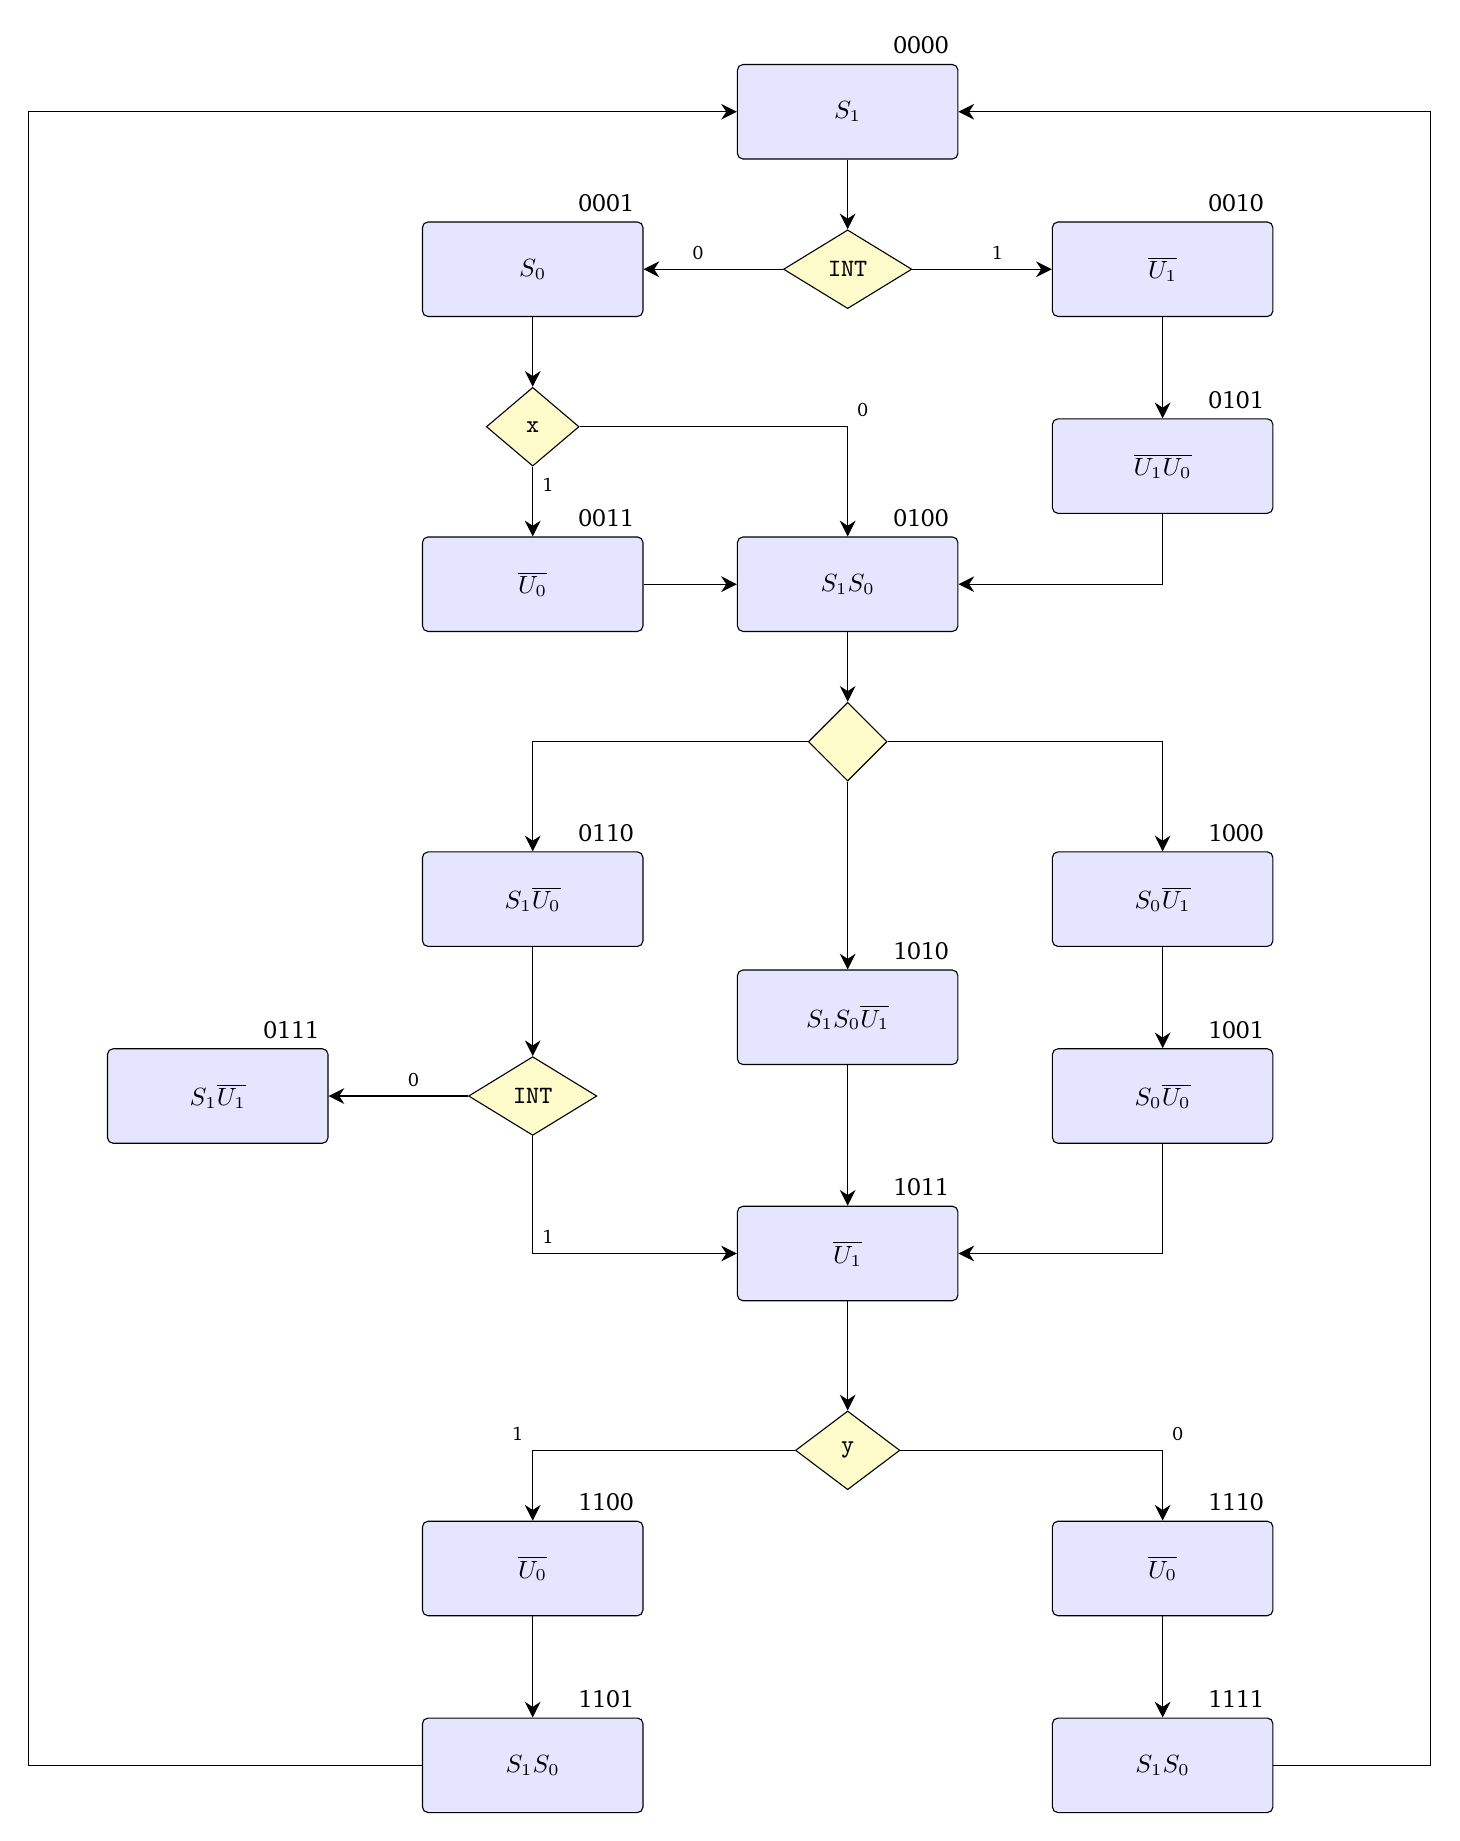
\begin{tikzpicture}[
        state/.style={draw, rounded corners=2pt, fill=blue!10, minimum width=2.8cm, minimum height=1.2cm, align=center, font=\small},
        decision/.style={draw, diamond, aspect=2.1, fill=yellow!20, minimum width=1cm, minimum height=1cm, align=center, font=\small},
        output/.style={draw, rounded corners=15pt, fill=gray!15, minimum width=2cm, minimum height=1cm, align=center, font=\small},
        >={Stealth[length=2mm,width=2mm]}
    ]
        \node[state, label={[anchor=south east, font=\small]north east:{0000}}] (E0) at (0,0) {$S_1$};
        \node[decision] (D0) at (0,-2) {\texttt{INT}};
        \node[state, label={[anchor=south east, font=\small]north east:{0001}}] (E1) at (-4,-2) {$S_0$};
        \node[decision] (D1) at (-4,-4) {\texttt{x}};
        \node[state, label={[anchor=south east, font=\small]north east:{0010}}] (E2) at (4,-2) {$\overline{U_1}$};
        \node[state, label={[anchor=south east, font=\small]north east:{0011}}] (E3) at (-4,-6) {$\overline{U_0}$};
        \node[state, label={[anchor=south east, font=\small]north east:{0100}}] (E4) at (0,-6) {$S_1S_0$};
        \node[state, label={[anchor=south east, font=\small]north east:{0101}}] (E5) at (4,-4.5) {$\overline{U_1}\overline{U_0}$};
        \node[decision] (T0) at (-0,-8) {};
        \node[state, label={[anchor=south east, font=\small]north east:{0110}}] (E6) at (-4,-10) {$S_1\overline{U_0}$};
        \node[state, label={[anchor=south east, font=\small]north east:{1000}}] (E8) at (4,-10) {$S_0\overline{U_1}$};
        \node[state, label={[anchor=south east, font=\small]north east:{0111}}] (E7) at (-8,-12.5) {$S_1\overline{U_1}$};
        \node[state, label={[anchor=south east, font=\small]north east:{1001}}] (E9) at (4,-12.5) {$S_0\overline{U_0}$};
        \node[state, label={[anchor=south east, font=\small]north east:{1010}}] (E10) at (0,-11.5) {$S_1S_0\overline{U_1}$};
        \node[state, label={[anchor=south east, font=\small]north east:{1011}}] (E11) at (0,-14.5) {$\overline{U_1}$};
        \node[state, label={[anchor=south east, font=\small]north east:{1100}}] (E12) at (-4,-18.5) {$\overline{U_0}$};
        \node[state, label={[anchor=south east, font=\small]north east:{1101}}] (E13) at (-4,-21) {$S_1S_0$};
        \node[state, label={[anchor=south east, font=\small]north east:{1110}}] (E14) at (4,-18.5) {$\overline{U_0}$};
        \node[state, label={[anchor=south east, font=\small]north east:{1111}}] (E15) at (4,-21) {$S_1S_0$};
        \node[decision] (D2) at (0,-17) {\texttt{y}};
        \node[decision] (D3) at (-4,-12.5) {\texttt{INT}};

        \draw[->] (E0) -- (D0);
        \draw[->] (D0) -- node[above left, font=\scriptsize] {0} (E1);
        \draw[->] (D0) -- node[above right, font=\scriptsize] {1} (E2);
        \draw[->] (E1) -- (D1);
        \draw[->] (D1) -- node[above right, font=\scriptsize] {1} (E3);
        \draw[->] (D1) -| node[above right, font=\scriptsize] {0} (E4);
        \draw[->] (E2) -- (E5);
        \draw[->] (E3) -- (E4);
        \draw[->] (E5) |- (E4);
        \draw[->] (E4) -- (T0);
        \draw[->] (T0) -| node[above left, font=\scriptsize] {} (E6);
        \draw[->] (T0) -| node[above right, font=\scriptsize] {} (E8);
        \draw[->] (T0) -- node[above right, font=\scriptsize] {} (E10);
        \draw[->] (E6) -- (D3);
        \draw[->] (D3) -- node[above right, font=\scriptsize] {0} (E7);
        \draw[->] (D3) |- node[above right, font=\scriptsize] {1} (E11);
        \draw[->] (E8) -- (E9);
        \draw[->] (E9) |- (E11);
        \draw[->] (E10) -- (E11);
        \draw[->] (E11) -- (D2);
        \draw[->] (D2) -| node[above left, font=\scriptsize] {1} (E12);
        \draw[->] (D2) -| node[above right, font=\scriptsize] {0} (E14);
        \draw[->] (E12) -- (E13);
        \draw[->] (E14) -- (E15);
        \draw[->] (E13.west) -- ++(-5,0) |- (E0);
        \draw[->] (E15.east) -- ++(2,0) |- (E0);
    \end{tikzpicture}
    \end{adjustbox}
    \caption{Carta ASM de 14 estados con entradas \texttt{INT} y \texttt{Qaux}.}
    \label{fig:carta_asm_14_limpia}
\end{figure}

\subsection*{2. Diseño de la lógica interna.}

Diseñe la lógica interna para que su secuenciador pueda ejecutar las instrucciones descritas anteriormente. Obtenga el contenido de la memoria de SU CARTA ASM para implementarlo en su secuenciador. Utilice el simulador para probar su implementación.

\subsection*{3. Simulación en Waveform}

Demuestre el correcto funcionamiento de su carta ASM SIMULANDOLO EN WAVEFORM y mostrándola a la profesora en el laboratorio.

\section*{Conclusiones}

\subsection*{Andrea Saldaña Navarrete - 320206384}


\subsection*{Hansel Yael Tepal Briseño - 320078282}


\subsection*{Luis Antonio Ugartechea González - 320223822}


\newpage
\section{Bibliografía}

% En formato IEEE

\begin{biblio}
	\hypertarget{1-diana-karen}{}
	\item D. K. Pérez Pérez, ``Reporte Construcción de Máquinas de Estados Usando Memorias'', Laboratorio de Organización y Arquitectura de Computadoras, Facultad de Ingeniería, Universidad Nacional Autónoma de México, Semestre 2027-1, 2026.
	\hypertarget{2-facultad-ingenieria}{}
	\item Facultad de Ingeniería, ``Capítulo III: Construcción de máquinas de estados usando memorias'', Apuntes de Arquitectura de Computadoras, Universidad Nacional Autónoma de México (UNAM). [En línea]. Disponible en: \url{https://biorobotics.fi-p.unam.mx/wp-content/uploads/Courses/arquitectura_de_computadoras/2021-1/lecciones/Leccion_3_arquitectura_de_computadoras_2021_1.pdf}
	% \hypertarget{3-savage}{}
	\item J. Savage, \textit{Diseño de Microprocesadores}, Facultad de Ingeniería, Universidad Nacional Autónoma de México (UNAM). [En línea]. Disponible en: \url{http://profesores.fi-b.unam.mx/luist/archivos/MicroprocesadoresSavage.pdf}
\end{biblio}

\end{document}
